%%%%%%%%%%%%%%%%%%%%%%%%%%%%%%%%%%%%%%%%%
% Short Sectioned Assignment LaTeX Template Version 1.0 (5/5/12)
% This template has been downloaded from: http://www.LaTeXTemplates.com
% Original author:  Frits Wenneker (http://www.howtotex.com)
% License: CC BY-NC-SA 3.0 (http://creativecommons.org/licenses/by-nc-sa/3.0/)
%%%%%%%%%%%%%%%%%%%%%%%%%%%%%%%%%%%%%%%%%

%----------------------------------------------------------------------------------------
%	PACKAGES AND OTHER DOCUMENT CONFIGURATIONS
%----------------------------------------------------------------------------------------

\documentclass[paper=a4, fontsize=11pt]{scrartcl} % A4 paper and 11pt font size

% ---- Entrada y salida de texto -----

\usepackage[T1]{fontenc} % Use 8-bit encoding that has 256 glyphs
\usepackage[utf8]{inputenc}
\usepackage{fourier} % Use the Adobe Utopia font for the document - comment this line to return to the LaTeX default

% ---- Idioma --------

\usepackage[spanish, es-tabla]{babel} % Selecciona el español para palabras introducidas automáticamente, p.ej. "septiembre" en la fecha y especifica que se use la palabra Tabla en vez de Cuadro

% ---- Otros paquetes ----

\usepackage{url} % ,href} %para incluir URLs e hipervínculos dentro del texto (aunque hay que instalar href)
\usepackage{amsmath,amsfonts,amsthm} % Math packages
%\usepackage{graphics,graphicx, floatrow} %para incluir imágenes y notas en las imágenes
\usepackage{graphics,graphicx, float} %para incluir imágenes y colocarlas
\usepackage{epstopdf}
\usepackage[gen]{eurosym} %para incluir el símbolo del euro
\usepackage{cite} %para incluir citas del archivo <nombre>.bib
%\graphicspath{/images}

% Para hacer tablas comlejas
%\usepackage{multirow}
%\usepackage{threeparttable}

%\usepackage{sectsty} % Allows customizing section commands
%\allsectionsfont{\centering \normalfont\scshape} % Make all sections centered, the default font and small caps

\usepackage{fancyhdr} % Custom headers and footers
\pagestyle{fancyplain} % Makes all pages in the document conform to the custom headers and footers
\fancyhead{} % No page header - if you want one, create it in the same way as the footers below
\fancyfoot[L]{} % Empty left footer
\fancyfoot[C]{} % Empty center footer
\fancyfoot[R]{\thepage} % Page numbering for right footer
\renewcommand{\headrulewidth}{0pt} % Remove header underlines
\renewcommand{\footrulewidth}{0pt} % Remove footer underlines
\setlength{\headheight}{13.6pt} % Customize the height of the header

\numberwithin{equation}{section} % Number equations within sections (i.e. 1.1, 1.2, 2.1, 2.2 instead of 1, 2, 3, 4)
\numberwithin{figure}{section} % Number figures within sections (i.e. 1.1, 1.2, 2.1, 2.2 instead of 1, 2, 3, 4)
\numberwithin{table}{section} % Number tables within sections (i.e. 1.1, 1.2, 2.1, 2.2 instead of 1, 2, 3, 4)

\setlength\parindent{0pt} % Removes all indentation from paragraphs - comment this line for an assignment with lots of text

\newcommand{\horrule}[1]{\rule{\linewidth}{#1}} % Create horizontal rule command with 1 argument of height


%----------------------------------------------------------------------------------------
%	TÍTULO Y DATOS DEL ALUMNO
%----------------------------------------------------------------------------------------

\title{
\normalfont \normalsize
\textsc{\textbf{Ingeniería de Servidores (2016-2017)} \\ Grado en Ingeniería Informática \\ Universidad de Granada} \\ [25pt] % Your university, school and/or department name(s)
\horrule{0.5pt} \\[0.4cm] % Thin top horizontal rule
\huge Memoria Práctica 3 \\ % The assignment title
\horrule{2pt} \\[0.5cm] % Thick bottom horizontal rule
}

\author{Adrián Morente Gabaldón} % Nombre y apellidos

\date{\normalsize\today} % Incluye la fecha actual

%----------------------------------------------------------------------------------------
% DOCUMENTO
%----------------------------------------------------------------------------------------

\begin{document}

\maketitle % Muestra el Título

\newpage %inserta un salto de página

\tableofcontents % para generar el índice de contenidos

\newpage

\listoffigures

\listoftables

\newpage


\section{Seleccione, instale y ejecute uno, comente los resultados. \textbf{Atención}: no es lo mismo un benchmark que una suite, instale un benchmark.}


\section{De los parámetros que le podemos pasar al comando ¿Qué significa -c 5? ¿Y -n 100? Monitorice la ejecución de ab contra alguna máquina (cualquiera) ¿cuántas ``tareas'' crea ab en el cliente?}
Apache Benchmark es uno de los benchmarks para servidores web más populares. Se ejecuta con el comando \textit{ab}, y si probamos a hacerlo sin haberlo instalado antes, obtendremos la siguiente salida en la terminal:
\begin{figure}[H]
	\centering
	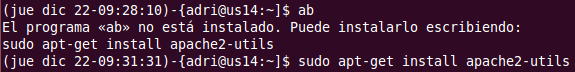
\includegraphics[scale=1]{ab-install}
	\caption{Ejecución fallida de ab seguida de su instalación. - Adrián Morente Gabaldón [22/12/2016]}
	\label{figura1}
\end{figure}
Esto nos indica que dicho programa no está instalado, y nos sugiere el nombre del paquete donde podemos encontrarlo. Acto seguido, vemos el comando para su instalación, que ejecutamos.
A continuación, podemos pasar a ejecutarlo con cualesquiera de sus opciones que deseemos, las cuales podemos consultar a través de su manual en la terminal, o en la propia documentación oficial de Apache \cite{ab-help}. Para este caso práctico, lo ejecutaremos de la forma \textbf{\textit{ab -c 5 -n 100}} pero antes, veamos que significan estas dos opciones:
\begin{figure}[H]
	\centering
	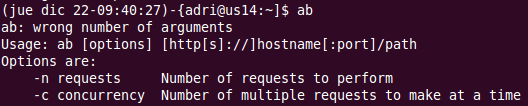
\includegraphics[scale=1]{ab-options}
	\caption{Parte de las opciones propuestas para la ejecución de ab. - Adrián Morente Gabaldón [22/12/2016]}
	\label{figura2}
\end{figure}
\begin{itemize}
	\item \textbf{-c 5}: \textit{``Number of multiple requests to make at a time''}; esto es, el número de hebras concurrentes que lanza el programa para los tests realizados. En este caso, veremos que lanza cinco hebras.
	\item \textbf{-n 10}: \textit{``Number of requests to perform''}; esto es, el número de consultas de prueba que realizará ab al servidor; (diez en este caso).
\end{itemize}
Pasemos ahora a ejecutar \textit{ab} contra la máquina de Ubuntu Server. Como vemos en el manual antes mencionado, se ejecuta con la siguiente estructura:
\begin{verbatim}
	ab [opciones] [http[s]://]hostname[:puerto]/ruta 
	POR EJEMPLO --> ab -c 5 -n 10 http://localhost/
\end{verbatim}
Aunque en el enunciado de la pregunta sugiere el uso de 5 hebras y 10 consultas, aumentaremos en gran medida este último número, ya que con solo 10 consultas el fin de la ejecución es inmediato; y lo que queremos realizar es una ejecución de larga duración para poder \textit{espiar} esta ejecución desde otra terminal con \textbf{htop} y así ver el número de tareas que crea ab. Realizaremos 500.000 consultas con 20 hebras a modo de ejemplo:
\begin{figure}[H]
	\centering
	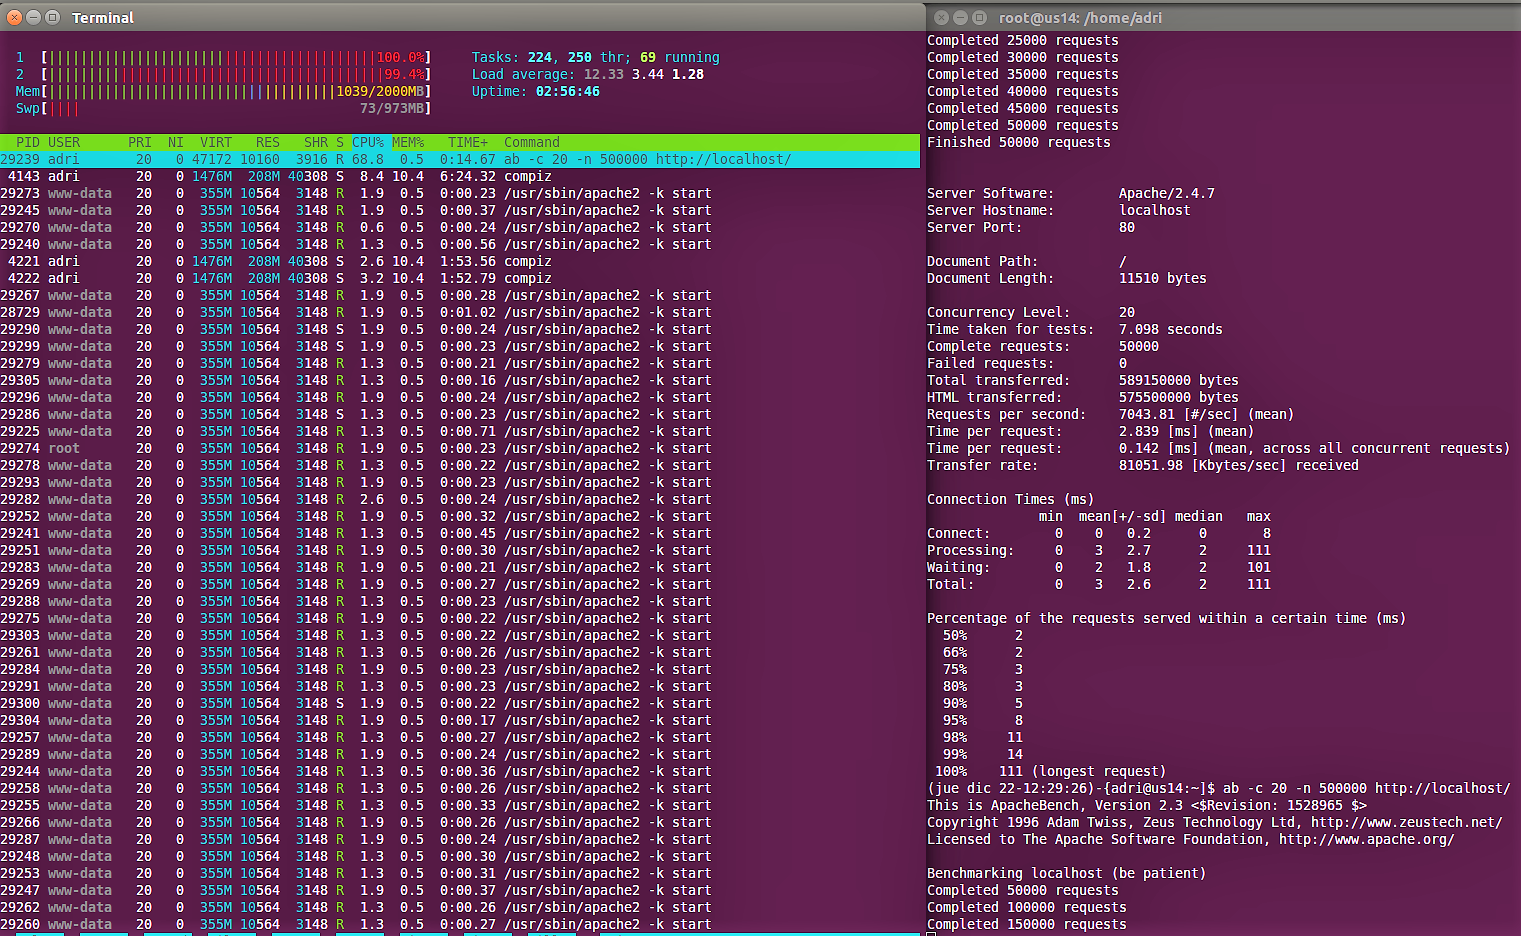
\includegraphics[scale=0.4]{ab-exec}
	\caption{Ejecución de ab contra Ubuntu Server y visualización de las tareas con htop. - Adrián Morente Gabaldón}
	\label{figura3}
\end{figure}
En la ventana de la izquierda, resaltado en azul podemos ver la(s) tarea(s) creadas por ab. Como vemos, tan solo crea \textbf{una} tarea real, ya que la concurrencia de las hebras que asignamos las ejecuta paralela o concurrentente de forma interna en su propio código; pero no crea hebras realmente concurrentes ejecutadas directamente en el procesador.
Con htop podemos ver el descriptor de proceso, el porcentaje de CPU y el tiempo empleado hasta el momento. Finalmente, la ejecución de ab con dichas opciones terminó tal que así, con 72 segundos empleados:
\begin{figure}[H]
	\centering
	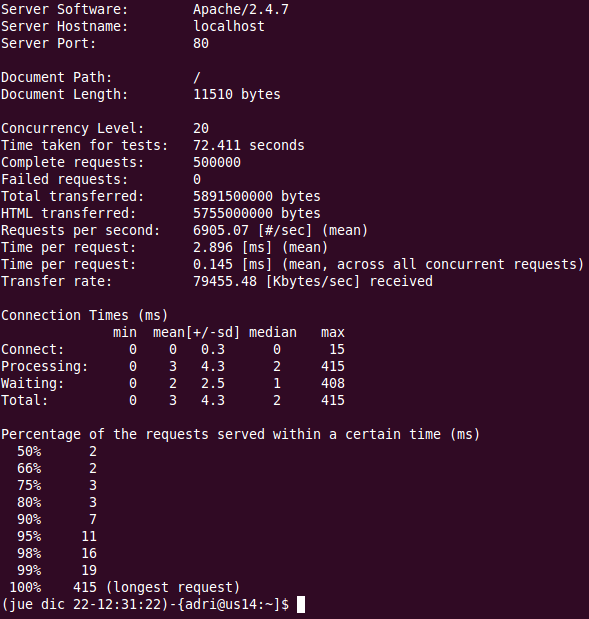
\includegraphics[scale=0.4]{ab-ubuntu}
	\caption{Ejecución de ab contra Ubuntu Server para 20 hebras y 500.000 consultas. - Adrián Morente Gabaldón [22/12/2016]}
	\label{figura4}
\end{figure}


\section{Ejecute ab contra las tres máquinas virtuales (desde el SO anfitrión a las máquinas virtuales de la red local) una a una (arrancadas por separado). ¿Cuál es la que proporciona mejores resultados? Muestre y coméntelos. (Use como máquina de referencia Ubuntu Server para la comparativa).}


\section{Instale y siga el tutorial en \href{http://jmeter.apache.org/usermanual/build-web-test-plan.html}{http://jmeter.apache.org/usermanual/build-web-test-plan.html} realizando capturas de pantalla y comentándolas. En vez de usar la web de jmeter, haga el experimento usando sus máquinas virtuales ¿coincide con los resultados de ab?}
	\subsection{Instalación de JMeter}
	Para esta prueba, utilizaremos otra vez Ubuntu Server. Empezaremos instalando JMeter según dictan en su web oficial \cite{jmeter-install}, que puede ser de varias formas, como veremos a continuación:
	\begin{itemize}
		\item Mediante el clonado y compilado del código fuente a través de \emph{Git/GitHub}.
		\item Mediante la descarga del código fuente más reciente en formato \emph{tar.gz} y posterior compilado del mismo.
		\item Mediante la descarga y ejecución de los binarios ya pre-compilados; que será la opción que elegiremos en este caso.
		\item Mediante la descarga e instalación desde los repositorios oficiales de Ubuntu.
	\end{itemize}
	En este caso práctico, optaremos por la última alternativa, ya que como sabemos, la instalación a través de terminal desde repositorios instala las dependencias necesarias y nos mantiene al tanto de las actualizaciones que se vayan sucediendo para el paquete instalado. Usaremos el comando \textbf{sudo apt-get install jmeter}, como nos indica la terminal de Ubuntu al intentar ejecutar JMeter sin instalarlo. Hecho esto, deberemos esperar a que termine de instalar cerca de unos 100MiB, ya que instalará dependencias grandes como los paquetes de Java 7, por ejemplo.
		
	Una vez instalado JMeter en Ubuntu Server, podemos lanzarlo simplemente con el comando \textbf{\$ \textit{jmeter}}, y veremos la siguiente interfaz gráfica:
	\begin{figure}[H]
		\centering
		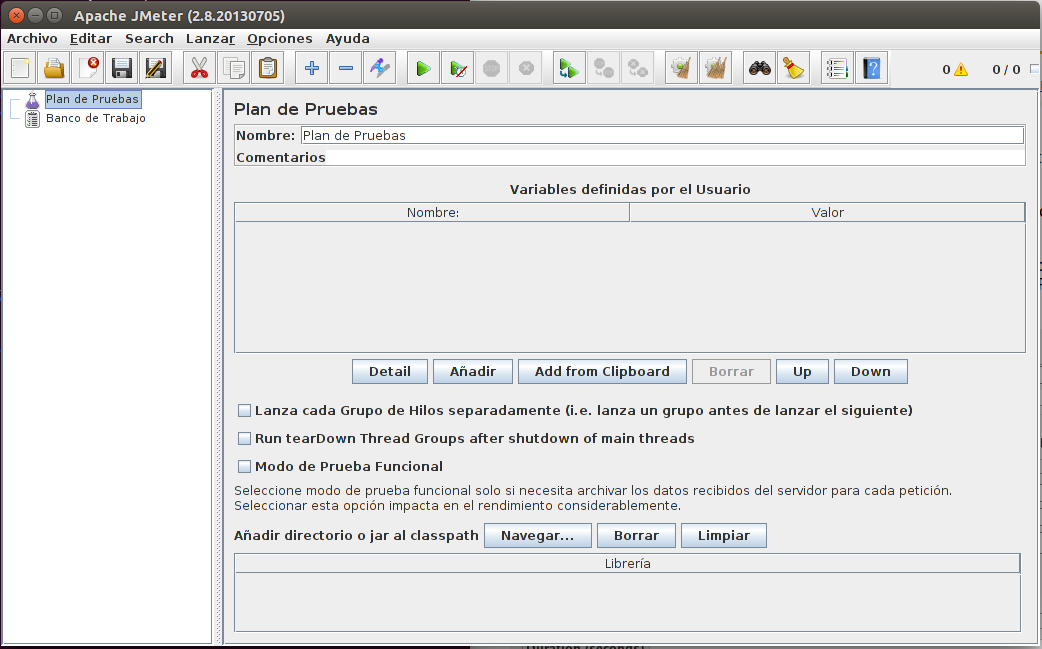
\includegraphics[scale=0.4]{jmeter-interface}
		\caption{Interfaz gráfica del programa Apache JMeter en Ubuntu Server. - Adrián Morente Gabaldón [22/12/2016]}
		\label{figura5}
	\end{figure}
	
	\subsection{Tutorial de Apache JMeter}
	Pasemos ahora a realizar y comentar el tutorial aportado en la web oficial \cite{ab-tutorial}; que consta de las siguientes partes:
	\begin{enumerate}
		\item \textbf{Descripción}: aprenderemos a crear un \emph{``Test Plan''} para testear un sitio web. Crearemos cinco usuarios, que enviarán dos consultas cada uno al servidor HTTP de la página web, dos veces. Es decir: (5 usuarios) x (2 peticiones) x (2 veces) = 20 peticiones al servidor de HTTP; sin embargo, más adelante veremos que son pocas muestras. Aunque en el tutorial se utiliza la página de JMeter para dichas consultas; en nuestro caso usaremos las páginas ofrecidas por nuestras máquinas virtuales. 
		
		\item \textbf{Adición de usuarios}: para empezar, añadiremos un nuevo Plan de Pruebas tal y como indica el tutorial:
		\begin{figure}[H]
			\centering
			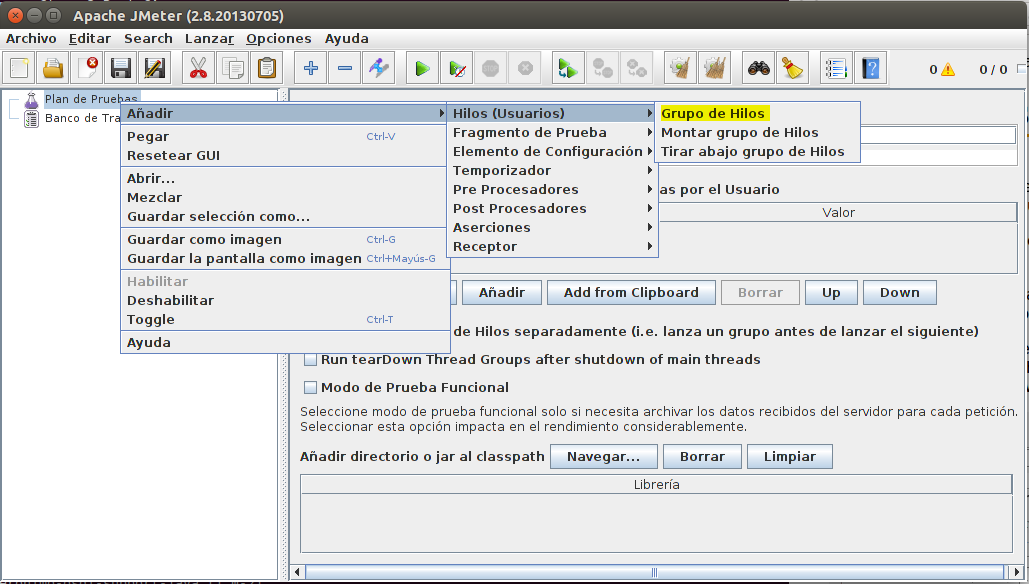
\includegraphics[scale=0.4]{jmeter-threadgroup}
			\caption{Creación de un nuevo grupo de hebras de ejecución. - Adrián Morente Gabaldón [22/12/2016]}
			\label{figura7}
		\end{figure}
		Empezaremos creando 5 usuarios (hilos o hebras) y ajustando el \emph{Periodo de Subida} a 1 segundo, que será el retardo con el que se lanzará cada hebra. Además, pondremos el \emph{Contador del bucle} a 2, que serán las veces que realizaremos las consultas, como mencionamos previamente. Si no quisiéramos un número determinado de ejecuciones, podríamos marcar la casilla \emph{Sin fin} y parar dicha ejecución cuando lo estimásemos oportuno. La configuración del test quedaría tal que así:
		\begin{figure}[H]
			\centering
			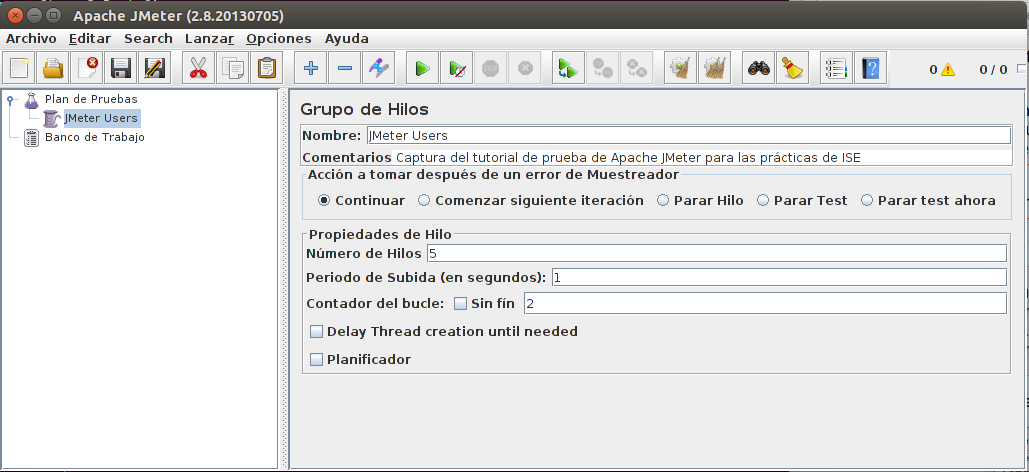
\includegraphics[scale=0.4]{jmeter-users}
			\caption{Configuración del Plan de Pruebas creado para el tutorial de Apache JMeter. - Adrián Morente Gabaldón [22/12/2016]}
			\label{figura6}
		\end{figure}
	
		\item \textbf{Creación de tareas}: ya que tenemos los usuarios (realmente hebras que los simbolizan), pasaremos a crear las tareas que desempeñarán éstos. Para empezar, crearemos un nuevo grupo de tareas del tipo \emph{Valores por defecto para petición HTTP}:
		\begin{figure}[H]
			\centering
			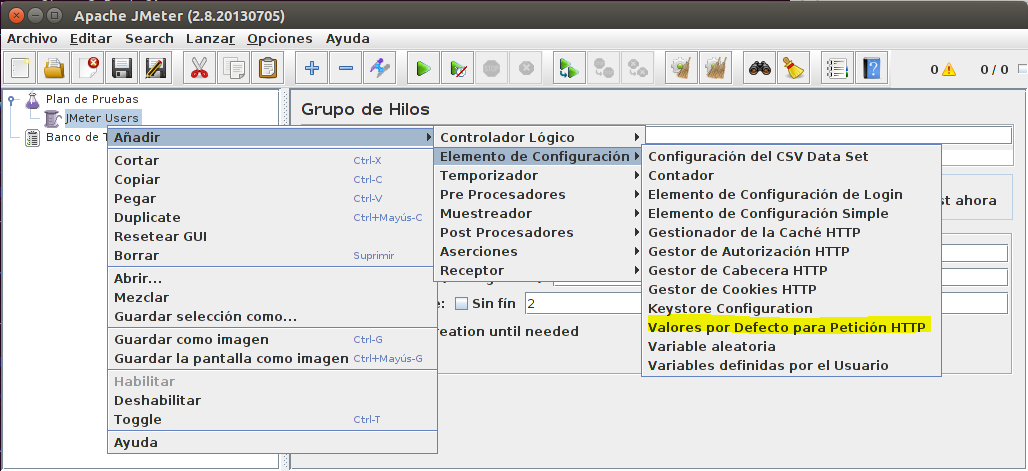
\includegraphics[scale=0.4]{jmeter-http}
			\caption{Creación de un nuevo grupo de tareas para el Plan creado anteriormente. - Adrián Morente Gabaldón [22/12/2016]}
			\label{figura8}
		\end{figure}
		Una vez creado, dejaremos todos los valores en blanco excepto el correspondiente a \emph{Nombre de Servidor o IP}, a cuyo campo asignaremos el valor de la IP a la que deseamos acceder (la propia de Ubuntu Server, en mi caso). La configuración quedaría de la siguiente forma:
		\begin{figure}[H]
			\centering
			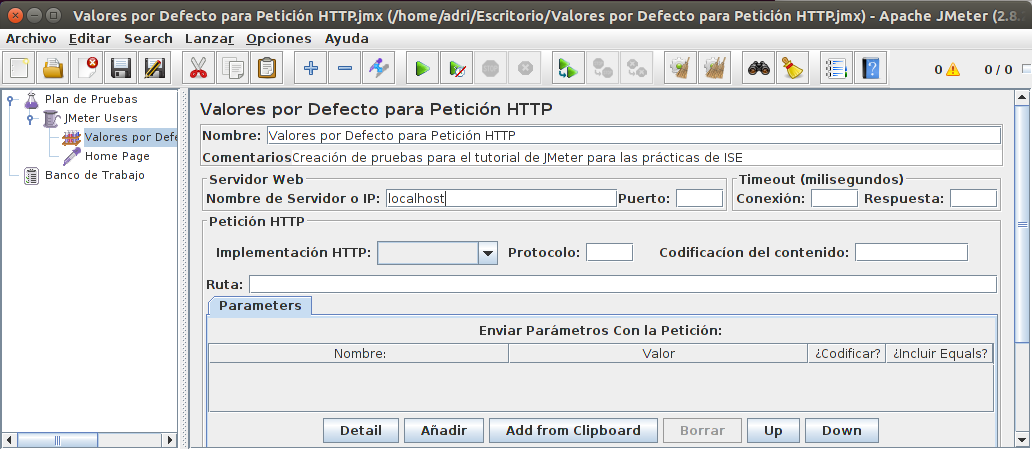
\includegraphics[scale=0.4]{jmeter-address}
			\caption{Asignación de la IP a consultar para los usuarios del nuevo Plan de Pruebas de JMeter. - Adrián Morente Gabaldón [22/12/2016]}
			\label{figura9}
		\end{figure}
	
		\item \textbf{Soporte para cookies}: la gran mayoría de las páginas web que consultamos hoy en día contienen cookies, que son pequeños depósitos de datos que permanecen almacenados localmente en el cliente para una mejor experiencia en la visualización y ejecución del contenido ofrecido en las webs que visita. En este caso, no añadiremos este soporte ya que las páginas que visualizaremos serán sencillas, estáticas y sin aplicaciones interactivas.
		
		\item \textbf{Adición de peticiones HTTP}: como anticipamos antes, queremos realizar consultas a la página web ofrecida por Ubuntu Server. Para ello, en JMeter deberemos añadir las consultas que deseamos hacer. Para ello, crearemos un nuevo apartado de \emph{Petición HTTP} de la forma que indicada el tutorial; tal que así:
		\begin{figure}[H]
			\centering
			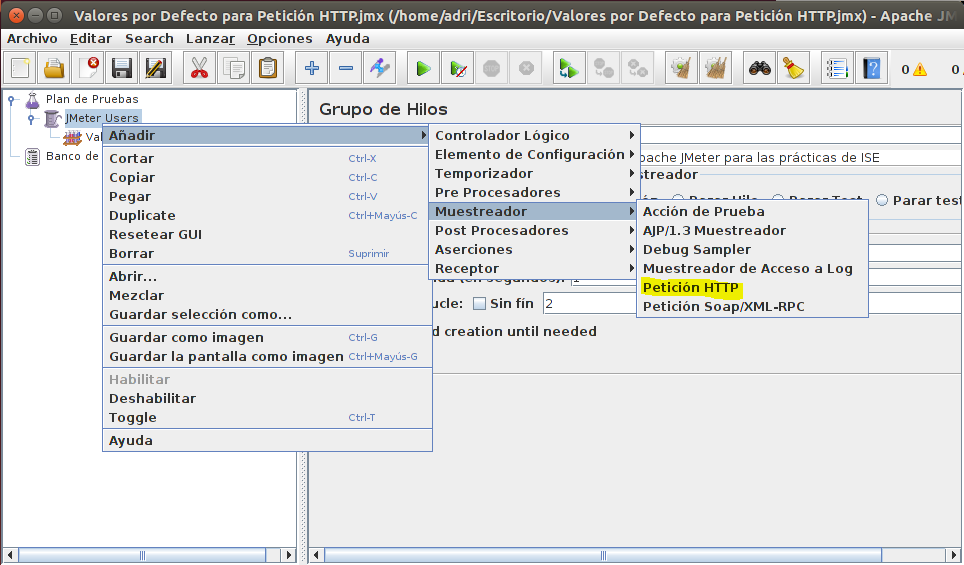
\includegraphics[scale=0.4]{jmeter-requests}
			\caption{Creación de peticiones HTTP para las pruebas de Apache JMeter. - Adrián Morente Gabaldón [22/12/2016]}
			\label{figura10}
		\end{figure}
		Para rellenar los campos, modificaremos el nombre de la petición, y fijaremos el directorio padre en la ruta de la petición HTTP. Para la segunda consulta, deberemos crear otro archivo \emph{Petición HTTP}. Sin embargo, en el tutorial de JMeter nos sugieren una ruta existente en su servidor, pero como utilizaremos nuestra página web, necesitaremos crear otro archivo \emph{.html} para dicha consulta. Para satisfacer esto, accederemos al directorio del que Apache2 obtiene el contenido a ofrecer en el servidor web, crearemos un nuevo directorio y copiaremos el antiguo index.html como un nuevo archivo, cambiando también su título. Acto seguido, obviamente tendremos que reiniciar el servicio:
		\begin{figure}[H]
			\centering
			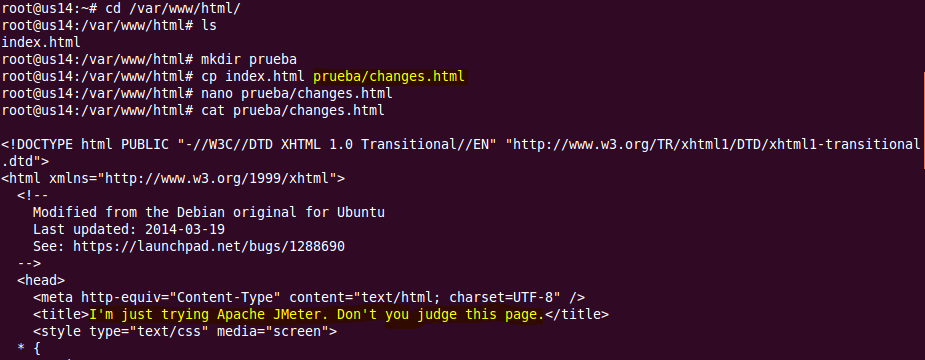
\includegraphics[scale=0.4]{jmeter-changes}
			\caption{Creación de una segunda página .html para las pruebas de Apache JMeter. - Adrián Morente Gabaldón [22/12/2016]}
			\label{figura11}
		\end{figure}
		Para verificar que el servidor web ofrece esta nueva página hagamos un pequeño inciso antes de avanzar:
		\begin{figure}[H]
			\centering
			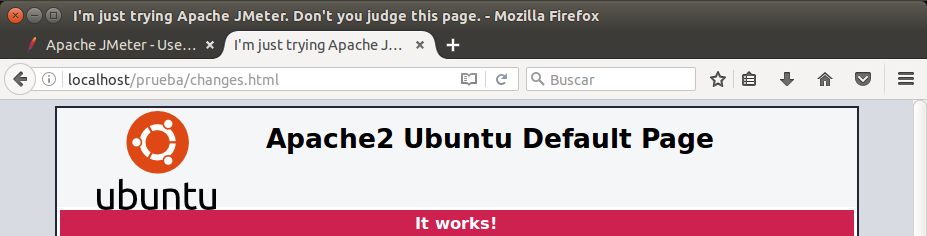
\includegraphics[scale=0.4]{jmeter-newpage}
			\caption{Visualización de los cambios en la nueva página web del servidor. - Adrián Morente Gabaldón [22/12/2016]}
			\label{figura12}
		\end{figure}
		Para terminar con la adición de peticiones HTTP, crearemos la segunda y fijaremos la ruta que lleva a la página que acabamos de crear, quedando tal que así:
		\begin{figure}[H]
			\centering
			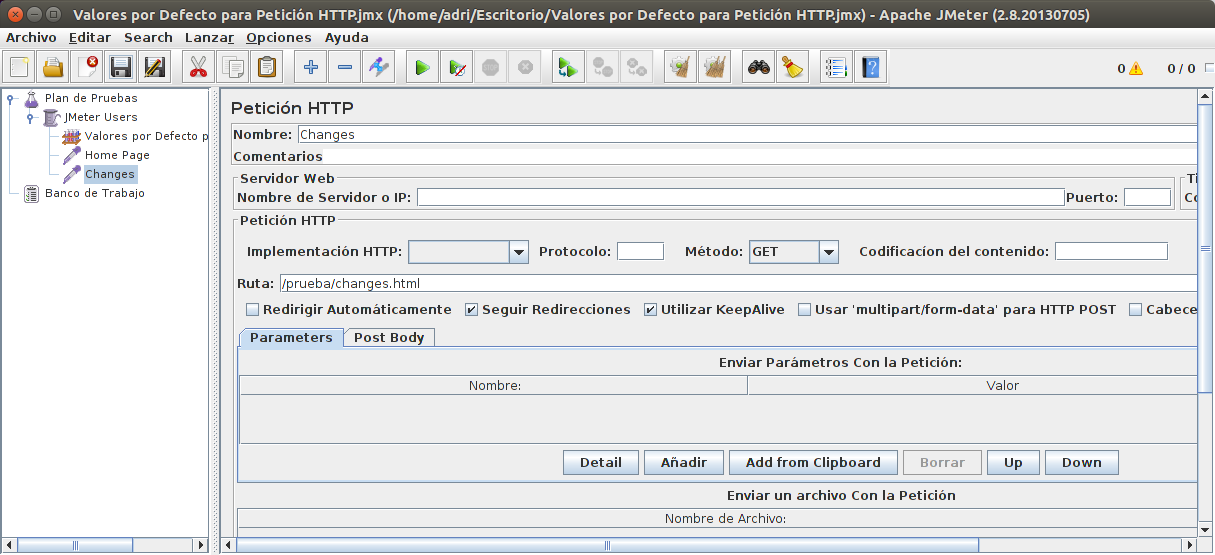
\includegraphics[scale=0.4]{jmeter-lasthttp}
			\caption{Visualización de la segunda petición HTTP a la página web del servidor. - Adrián Morente Gabaldón [22/12/2016]}
			\label{figura13}
		\end{figure}
	
		\item \textbf{Visualización de los datos}: para terminar, deberemos crear un \emph{Listener}, que será el encargado de recoger todos los resultados de las mediciones y representarlos de forma gráfica y más visual que una simple tabla de números. Una vez más, creamos dicha \emph{feature} siguiendo las instrucciones aportadas por el tutorial. Definiremos la ubicación donde se almacenará el archivo con dichos resultados y pediremos que nos muestre todos los datos referentes (Nº de muestras, media, mediana, etc.). Para 20 consultas, como dicta el tutorial, obtenemos una gráfica insulsa y sin apenas datos, de forma que no podemos interpretarlos y comentarlos. Dado esto, las realizaremos con 5000 usuarios, (o mejor dicho, hebras). Hecho esto, obtenemos la siguiente gráfica:
		\begin{figure}[H]
			\centering
			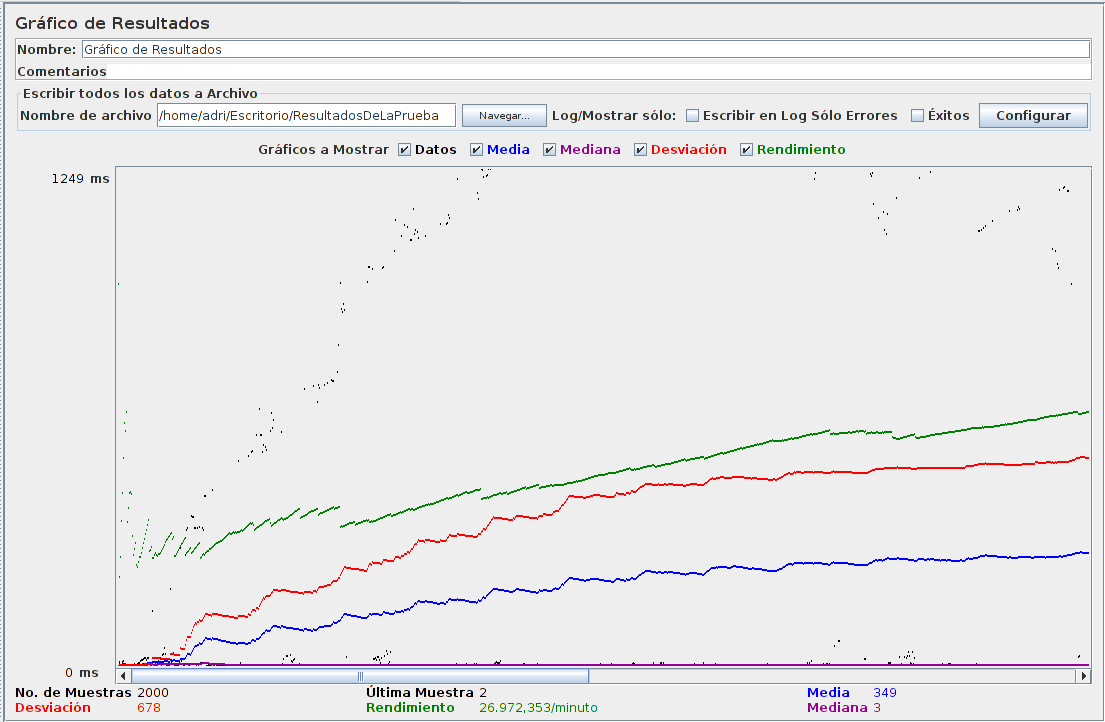
\includegraphics[scale=0.4]{jmeter-finalexec}
			\caption{Visualización de la gráfica resultante final del tutorial de JMeter. - Adrián Morente Gabaldón [22/12/2016]}
			\label{figura14}
		\end{figure}
		Para terminar, podemos apreciar que el rendimiento ofrecido es muy bueno, ya que el número de operaciones realizadas por minuto es muy alto. Además, según vemos en el valor de la última consulta, se han realizado todas en tan solo 2 segundos.
	\end{enumerate}


\section{Programe un benchmark usando el lenguaje que desee. El benchmark debe incluir: 1) Objetivo del benchmark. 2) Métricas (unidades, variables, puntuaciones, etc.). 3) Instrucciones para su uso. 4) Ejemplo de uso analizando los resultados.}



\bibliography{citas}
\bibliographystyle{plain}
\end{document}
